\chapter{Arquitetura do projeto}

O objetivo deste capítulo é descrever a parte de arquitetura do projeto.

\section{Representação Arquitetural}

A figura \ref{fig:arquitetura} apresenta o fluxo de dados da arquitetura.

\begin{figure}[ht]
	\centering
    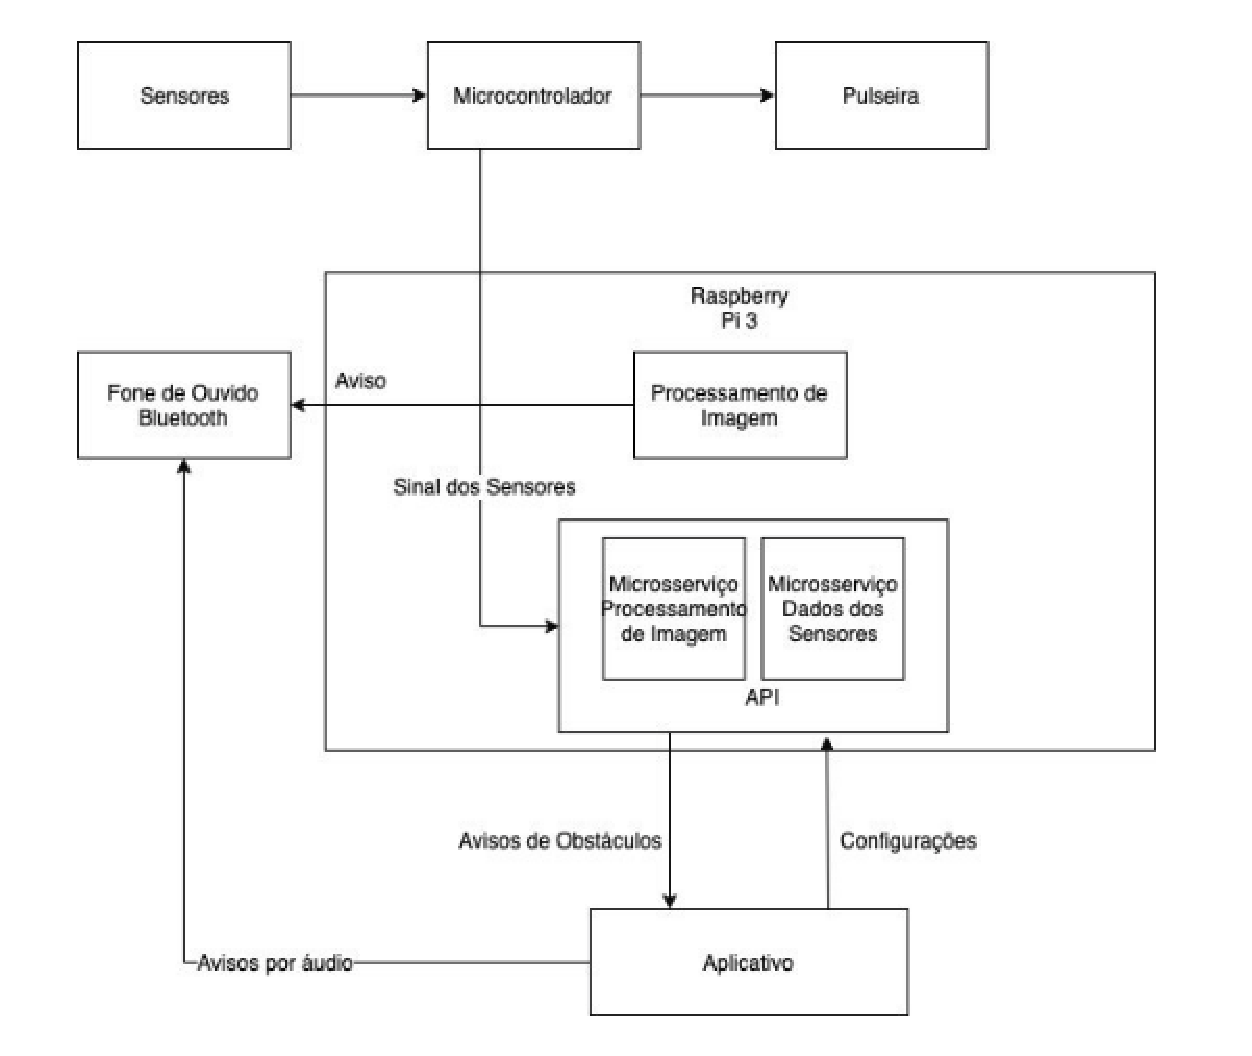
\includegraphics[keepaspectratio=true,scale=0.5]{figuras/arquitetura.eps}
    \caption[Arquitetura do projeto.]{Arquitetura do projeto. Fonte: Autor}
	\label{fig:arquitetura}
\end{figure}

O projeto possui uma Raspberry Pi 3 responsável por alocar os microsserviços de software para que possa ocorrer comunicação entre os dispositivos via WiFi. Os microsserviços envolvidos são o de reconhecimento da faixa de pedestre e o de reconhecimento de sinais dos sensores, nos quais permitem que esses dados possam ser reutilizados como boa prática de engenharia de software por meio de uma API pública. O fone de ouvido ou alto falante conectado via bluetooth pode ser tanto utilizado diretamente pela raspiberry, como pelo celular, escolhido na configuração de preferência do usuário.

\section{Restrições e Metas arquiteturais}

\begin{itemize}
    \item O projeto tem como software base o processamento de imagem para reconhecimento de faixa de pedestres, por conta disso, haverá um algoritmo;
    \item O projeto abrange um sistema de feedback por áudio;
    \item O aplicativo será desenvolvido para multiplataforma utilizando tecnologias como React Native, porém só será compilado na plataforma Android, devido ao prazo para cumprimento do projeto.
    \item A aplicação estará estruturada na arquitetura Model View Controller (MVC) comumente aplicada por aplicações mobile.
    \item O software de processamento de imagem será desenvolvido na linguagem Python 3.7 utilizando o framework OpenCV e Flask e estará associado a uma raspberry;
    \item Haverá um servidor utilizando o framework Flask para a comunicação via WiFi entre os dispositivos.
\end{itemize}

O sistema de identificação de faixa de pedestre será implementado para que em conjunto com o aplicativo e o fone de ouvido ou auto falante, informe ao usuário que foi identificada uma faixa de pedestre. Dessa forma, seguem as metas e restrições identificadas:

\begin{itemize}
    \item Será um sistema embarcado em uma raspberry para análise de vídeo, enviado pela câmera estrategicamente posicionada em um óculos.  A raspberry emitirá um comando para um microsserviço responsável pela interpretação e envio da mensagem em áudio para o fone de ouvido ou auto falante.
    \item O aplicativo se comunicará via WiFi com a raspberry, indicando a habilitação ou não de emissão de mensagem sonora.
\end{itemize}